%==============================================================================
%  DPU-Native Deployment of an Orthogonalization-Regularized FER Detector
%  on Zynq UltraScale+ (ZCU104)  --  FPGA implementation manuscript
%
%  INTEGRITY NOTE: Host-measurable result cells (FER2013 FP32 accuracy/macro-F1,
%  the fold-out delta, and the model-intrinsic workload/roofline quantities) are
%  populated from real runs. On-board cells that require the physical ZCU104
%  (resource utilization, timing closure, power, measured latency/FPS) remain
%  explicit placeholders ("--"). No measured value is invented. Vendor-documented
%  architectural constants (PG338, UG1267, device tables) are cited; formula-derived
%  theoretical values are labelled as such. On-board figure slots are marked
%  "pending board measurement".
%==============================================================================
\documentclass[onecolumn,journal]{IEEEtran}

\usepackage[T1]{fontenc}
\usepackage[utf8]{inputenc}
\usepackage{amsmath,amssymb,amsfonts}
\usepackage{mathtools}
\usepackage{bm}
\usepackage{graphicx}
\usepackage{booktabs}
\usepackage{multirow}
\usepackage{makecell}
\usepackage{array}
\usepackage{xcolor}
\usepackage[protrusion=true,expansion=false]{microtype}
\usepackage[ruled,vlined,linesnumbered]{algorithm2e}
\usepackage{tikz}
\usetikzlibrary{arrows.meta,positioning,calc,fit,backgrounds,shapes.geometric,%
  decorations.pathreplacing,patterns}
\usepackage[hidelinks]{hyperref}
\usepackage{url}
\usepackage{pifont}
\newcommand{\cmark}{\ding{51}}
\newcommand{\xmark}{\ding{55}}

% ---- colours ----
\definecolor{psblue}{RGB}{55,95,190}
\definecolor{plgreen}{RGB}{40,130,90}
\definecolor{dpuorange}{RGB}{220,120,20}
\definecolor{memgray}{RGB}{110,110,110}
\definecolor{orthoblue}{RGB}{30,120,160}

% ---- macros ----
\newcommand{\R}{\mathbb{R}}
\newcommand{\tbd}{\textcolor{gray}{--}}
\newcommand{\Conv}{\mathrm{Conv}}
\newcommand{\fmax}{f_{\mathrm{max}}}
\newcommand{\Ppeak}{P_{\mathrm{peak}}}

\begin{document}

\title{Folding Structure Out of the Datapath:\\
A DPU-Native FPGA Deployment Methodology\\
for a Real-Time Orthogonalization-Regularized\\
Facial-Emotion Detector on the Zynq UltraScale+ MPSoC}

\author{Olfa~Askri,~Saifeddine~Massoud,~and~Mohamed~Ali~Hajjaji%
\thanks{O.~Askri is with ENET'Com, National School of Electronics and
Telecommunications of Sfax, University of Sfax, Sfax, Tunisia, and also with the
Laboratory of Electronics and Microelectronics (E$\mu$E, LR99ES30), University of
Monastir, Monastir, Tunisia (e-mail: Olfa.Askri@esen.tn).}%
\thanks{S.~Massoud and M.~A.~Hajjaji are with the Laboratory of Electronics and
Microelectronics (E$\mu$E, LR99ES30), University of Monastir, Monastir, Tunisia.}%
\thanks{Corresponding author: O.~Askri. \textit{Co-author contact details and ORCIDs to
be completed prior to submission.}}}

\markboth{Manuscript --- Draft for Submission}%
{Askri \MakeLowercase{\textit{et al.}}: DPU-Native Deployment of an Orthogonalization-Regularized FER Detector}

\maketitle

%==============================================================================
\begin{abstract}
%==============================================================================
Modern convolutional accelerators for FPGAs, exemplified by the AMD/Xilinx Deep-Learning
Processing Unit (DPU), obtain their efficiency from a deliberately narrow contract: INT8
arithmetic, convolution-centric instructions, and no divisions, square roots, or
data-dependent recurrences on the datapath. Training-time innovations in deep learning
routinely violate this contract. This paper develops, end to end, a deployment
methodology for one such case: a real-time facial-emotion detector whose neck embeds a
differentiable Gram--Schmidt orthogonalization stage---an operator that is useful during
optimization and hostile to the accelerator at inference. Our central idea is
architectural rather than algorithmic: treat the offending structure as a
\emph{training-time regularizer} and fold it out of the exported inference graph, so
that the deployed network is composed exclusively of DPU-native operators. We formalize
the fold-out as a graph rewrite with an explicitly defined accuracy cost, present a
division-free Householder alternative whose normalization constants are folded into
per-channel scales at export time, and specify a hybrid processing-system/programmable-logic
schedule as the conservative fallback. The methodology is developed for the Zynq
UltraScale+ XCZU7EV on the ZCU104 evaluation platform with a B4096 DPU
(peak $4096$ operations per cycle; $1.229$~TOPS at $300$~MHz), under the Vitis~AI
quantization and compilation flow. We derive the complete metric framework---maximum
clock frequency from timing slack, resource utilization against device totals, roofline
throughput bounds, power decomposition, and energy per inference---with explicit
formulas and measurement procedures for each, and we structure the validation around
component-isolating experiments whose decisive quantity is the accuracy cost of the
folded graph against the full one. On FER2013, the host-side validation is complete:
the full-graph detector matches the unaugmented baseline
($71.9\%$ vs.\ $71.4\%$ top-1, $+0.8$ macro-F1 points), and the fold-out costs a
measured $\Delta_{\mathrm{fold}}=5.1$ accuracy points ($6.2$ macro-F1 points), of
which the division-free Householder route recovers roughly two-fifths at no
datapath cost. The model-intrinsic roofline analysis, computed from the compiled
operator graph, places all three routes firmly in the compute-bound regime
(arithmetic intensity $\approx\!266$ op/byte against a ridge of $64$ op/byte). In
keeping with research-integrity practice, the cells that require the physical board
(resource, timing, power, and measured latency) are explicitly marked pending; the
architectural constants, formulas, vendor-documented figures, and all host-measurable
results are complete, so that the remaining on-board experiments are decisive rather
than decorative.
\end{abstract}

\begin{IEEEkeywords}
FPGA, Zynq UltraScale+, deep-learning processing unit (DPU), hardware--software
co-design, INT8 quantization, facial emotion recognition, real-time inference,
Vitis AI, graph rewriting, energy efficiency.
\end{IEEEkeywords}

%==============================================================================
\section{Introduction}\label{sec:intro}
%==============================================================================
\IEEEPARstart{F}{ield}-programmable gate arrays occupy a specific niche in embedded
deep-learning inference: deterministic latency, watt-level power envelopes, and the
freedom to shape the memory system around the workload. For convolutional networks the
dominant deployment style on recent AMD/Xilinx devices is not a hand-written dataflow
circuit but an \emph{overlay}: a pre-implemented, instruction-programmable accelerator
--- the Deep-Learning Processing Unit (DPU) --- that the toolchain targets by compiling
the network into an instruction stream \cite{amd_pg338,amd_ug1414}. The overlay style
trades some peak efficiency for an enormous practical benefit: the programmable-logic
design is fixed, timing closure is done once, and iterating on the network requires no
hardware re-synthesis.

The efficiency of the overlay comes from a deliberately narrow operator contract. The
DPUCZDX8G executes INT8 multiply--accumulate work on a systolic convolution engine with
three axes of parallelism, supports a curated list of layer types, and offers no
division, no square root, and no data-dependent recurrence on the datapath
\cite{amd_pg338}. Networks that respect the contract compile to a single accelerator
subgraph and run at predictable throughput; networks that violate it are split, with the
offending operators falling back to the ARM processing system (PS), where a single
serialized operator can dominate end-to-end latency.

This paper is about what to do when a network worth deploying violates the contract
\emph{by design}. Our workload is a real-time facial-emotion detector for e-learning and
human--machine interaction: a YOLOv12 object detector \cite{tian2025yolov12} whose neck
is augmented with FLEO, a module that partitions features into per-emotion subspaces and
enforces their mutual orthogonality with a differentiable Gram--Schmidt pass, developed
in a companion manuscript \cite{askri2026fleo}. The orthogonalization demonstrably
belongs in the \emph{training} computation: it is the mechanism by which the network is
regularized toward separable emotion subspaces. At \emph{inference} it is a liability:
Gram--Schmidt requires a reciprocal square root per subspace, a division per projection,
and a sequential recurrence across subspaces --- three properties that individually
disqualify an operator from the DPU and jointly guarantee a PS fallback.

The resolution we develop is architectural, and its appeal is its simplicity. Rather
than porting the offending operator to hardware, we ask whether the \emph{effect} of the
operator survives in the trained weights when the operator itself is removed from the
exported graph. We call this the \emph{fold-out}: a graph rewrite applied at export time
that deletes the orthogonalization stage, leaving a network composed exclusively of
DPU-native operators --- $1{\times}1$ and $3{\times}3$ convolutions, pooling, sigmoid
gating, and elementwise arithmetic. The rewrite has a precisely defined accuracy cost,
which we elevate to the central measured quantity of the validation. Around this idea we
build the complete deployment methodology: the operator-compatibility analysis that
motivates it, a division-free Householder alternative for the case where inference-time
orthogonality must be retained, a hybrid PS/PL schedule as the conservative fallback,
the INT8 quantization workflow, and a fully explicit metric framework for timing, area,
power, throughput, and energy.

\paragraph*{Contributions} The paper makes the following contributions.
\begin{enumerate}
\item \textbf{An operator-contract analysis} that classifies every operator of the
augmented detector against the DPUCZDX8G instruction set and identifies, for each
non-native operator, the property that disqualifies it (division, square root, or
sequential recurrence) together with its mitigation (Section~\ref{sec:compat}).
\item \textbf{The fold-out methodology}: a formally stated export-time graph rewrite
that removes the training-time orthogonalization from the inference graph, with a
correctness discussion separating what the rewrite preserves exactly (the learned
weights, the gating branch, the residual path) from what it approximates (the
orthogonalized activations), and a definition of the fold-out accuracy delta
$\Delta_{\mathrm{fold}}$ as the decisive experiment, measured on FER2013 at
$\Delta_{\mathrm{fold}}=5.1$ accuracy points (Sections~\ref{sec:foldout}
and~\ref{sec:results}).
\item \textbf{A division-free structural alternative}: a Householder-product
orthogonalization whose normalization constants, being fixed after training, are folded
into per-channel scales at export --- turning a datapath division into a compile-time
constant and keeping the operator on the accelerator (Section~\ref{sec:householder}).
\item \textbf{A complete metric and validation framework} with explicit formulas for
maximum clock frequency from worst negative slack, resource utilization against device
totals, peak and effective throughput, roofline bounds, power decomposition, and energy
per inference, each tied to a concrete measurement procedure on the ZCU104
(Section~\ref{sec:metrics}).
\item \textbf{A reproducible experimental protocol with the host-measurable results
populated}: the FER2013 FP32 accuracy block (baseline, the three routes, and
$\Delta_{\mathrm{fold}}$) and the model-intrinsic workload/roofline placement are
reported from real runs, while the cells that require the physical board (resources,
timing, power, measured latency) are explicitly marked pending so that no unmeasured
value is reported (Sections~\ref{sec:setup} and~\ref{sec:results}).
\end{enumerate}

The remainder of the paper is organized as follows. Section~\ref{sec:related} reviews
the accelerator landscape and prior FPGA-based expression-recognition systems.
Section~\ref{sec:arch} describes the target platform and system architecture.
Section~\ref{sec:method} develops the deployment methodology.
Section~\ref{sec:metrics} derives the metric framework. Section~\ref{sec:setup}
specifies the experimental protocol, Section~\ref{sec:results} presents the results
templates, Section~\ref{sec:discussion} analyzes trade-offs and limitations, and
Section~\ref{sec:conclusion} concludes.

%==============================================================================
\section{Background and Related Work}\label{sec:related}
%==============================================================================

\subsection{FPGA acceleration of convolutional networks}
Two design styles dominate. \emph{Bespoke dataflow} designs synthesize a circuit per
network, streaming activations between layer-specific compute stages; FINN is the
canonical framework for aggressively quantized networks in this style
\cite{umuroglu2017finn}. \emph{Overlay} designs implement one general matrix/convolution
engine and program it per network; the DPUCZDX8G on Zynq UltraScale+ is the
production-grade representative \cite{amd_pg338}. Between these poles, a long line of
work established the analytical tools this paper relies on: Zhang \textit{et al.}
brought the roofline model to FPGA accelerator design, making explicit the interplay of
compute peak and memory bandwidth \cite{zhang2015optimizing}, and Qiu \textit{et al.}
demonstrated a full embedded-Zynq CNN deployment with fixed-point quantization and
bandwidth-conscious design \cite{qiu2016going}. Our work sits deliberately in the
overlay style: the contribution is not a new engine but a methodology for making a
structurally non-conforming network conform.

\subsection{Integer quantization for accelerators}
INT8 inference with per-tensor scale factors is the established accelerator interface;
Jacob \textit{et al.} formalized the affine-quantization arithmetic and the
quantization-aware-training procedure that recovers accuracy lost to rounding
\cite{jacob2018quantization}, and Krishnamoorthi's whitepaper systematized the
post-training and calibration options \cite{krishnamoorthi2018quantizing}. The Vitis~AI
flow constrains the quantizer further to hardware-friendly power-of-two scaling so that
rescaling reduces to bit shifts on the DPU \cite{amd_ug1414}. These constraints shape
Section~\ref{sec:quant}: operators whose dynamic range interacts badly with power-of-two
scales are exactly the ones the fold-out removes.

\subsection{Expression recognition on embedded FPGAs}
FPGA implementations of facial-expression recognition span a decade of styles.
Phan-Xuan \textit{et al.} implemented a compact CNN classifier on an FPGA platform with
hand-mapped layers \cite{phanxuan2019fpga}; Vinh and Vinh demonstrated an SoC-FPGA
expression-recognition system integrating detection and classification on Zynq
\cite{vinh2019soc}. Closest to our setting, Ando and Inoue deploy both a face detector
and an expression classifier on a single DPU with multi-threading, reporting a 25-FPS
standalone system and showing that CPU-side stages, not the accelerator, bound
throughput \cite{ando2025fer}. Our own prior work optimized a FER network for efficient
inference with a quantum-inspired metaheuristic \cite{askri2024qgoa}. What none of these
systems confronts is a network whose \emph{architecture} embeds an accelerator-hostile
operator by design; that gap --- structural training-time components on a
contract-constrained overlay --- is the one this paper addresses.

%==============================================================================
\section{System Architecture}\label{sec:arch}
%==============================================================================

\subsection{Target platform}
The target is the ZCU104 evaluation platform built around the Zynq UltraScale+
XCZU7EV-2FFVC1156 multiprocessor system-on-chip \cite{amd_ug1267}. The device pairs a
processing system (quad-core Arm Cortex-A53, dual-core Cortex-R5F, Mali-400 GPU, and a
hardened H.264/H.265 video codec unit) with a programmable-logic fabric of
$230{,}400$ LUTs, $460{,}800$ flip-flops, $312$ block-RAM tiles (36\,Kb),
$96$ UltraRAM blocks (288\,Kb), and $1{,}728$ DSP48E2 slices. The PS memory system is a
64-bit, 2\,GB DDR4 channel; at a transfer rate of $R$ mega-transfers per second its
theoretical peak bandwidth is
\begin{equation}
\beta_{\mathrm{DDR}} = R \times 8~\text{bytes} ,
\label{eq:bw}
\end{equation}
i.e. $19.2$~GB/s at DDR4-2400. Table~\ref{tab:platform} summarizes the platform;
Fig.~\ref{fig:system} shows the system architecture, including the power-monitoring
path used in Section~\ref{sec:metrics}.

\begin{table}[t]
\centering
\caption{Target platform summary (vendor-documented figures \cite{amd_ug1267}).}
\label{tab:platform}
\renewcommand{\arraystretch}{1.2}
\begin{tabular}{ll}
\toprule
Item & Value\\
\midrule
Board & ZCU104 evaluation kit\\
Device & Zynq UltraScale+ XCZU7EV-2FFVC1156\\
PS application cores & 4$\times$ Arm Cortex-A53\\
PS real-time cores & 2$\times$ Arm Cortex-R5F\\
PL logic & 230{,}400 LUTs; 460{,}800 FFs\\
PL memory & 312 BRAM36 (11\,Mb); 96 URAM (27\,Mb)\\
PL arithmetic & 1{,}728 DSP48E2\\
PS DRAM & 2\,GB DDR4, 64-bit channel\\
Accelerator & DPUCZDX8G, B4096, single core\\
\bottomrule
\end{tabular}
\end{table}

\begin{figure}[t]
\centering
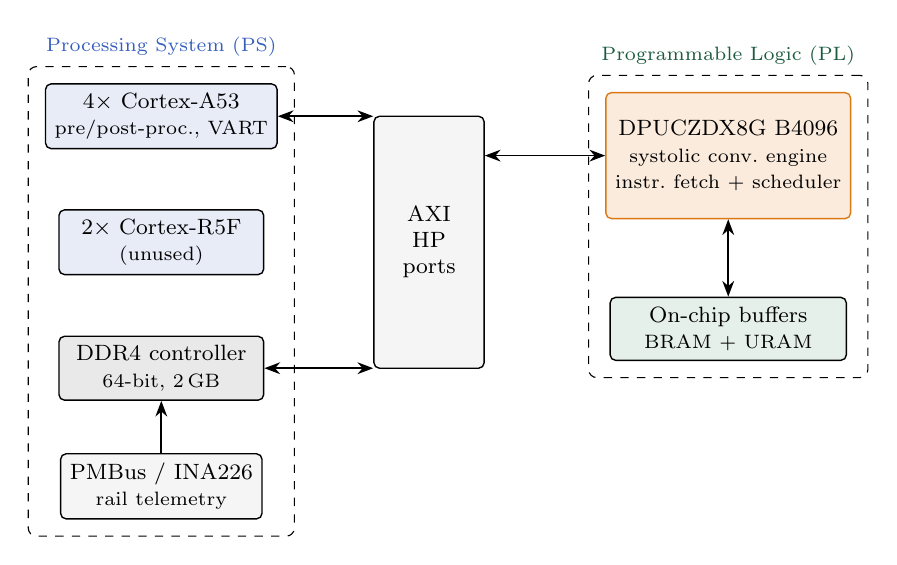
\begin{tikzpicture}[font=\footnotesize,>={Stealth[length=2mm]},
  blk/.style={draw,rounded corners=2pt,minimum height=8mm,align=center,line width=0.5pt},
  arr/.style={<->,line width=0.6pt}]
% PS side
\node[blk,fill=psblue!12,minimum width=26mm] (a53) at (0,1.1) {4$\times$ Cortex-A53\\\scriptsize pre/post-proc., VART};
\node[blk,fill=psblue!12,minimum width=26mm] (r5)  at (0,-0.5) {2$\times$ Cortex-R5F\\\scriptsize (unused)};
\node[blk,fill=memgray!15,minimum width=26mm] (ddr) at (0,-2.1) {DDR4 controller\\\scriptsize 64-bit, 2\,GB};
% Interconnect
\node[blk,fill=gray!8,minimum width=14mm,minimum height=32mm] (axi) at (3.4,-0.5) {AXI\\HP\\ports};
% PL side
\node[blk,fill=dpuorange!15,draw=dpuorange,minimum width=30mm,minimum height=16mm] (dpu) at (7.2,0.6)
  {DPUCZDX8G B4096\\\scriptsize systolic conv.\ engine\\\scriptsize instr.\ fetch + scheduler};
\node[blk,fill=plgreen!12,minimum width=30mm] (bram) at (7.2,-1.6) {On-chip buffers\\\scriptsize BRAM + URAM};
% power monitor
\node[blk,fill=gray!8,minimum width=22mm] (pmb) at (0,-3.6) {PMBus / INA226\\\scriptsize rail telemetry};
% edges
\draw[arr] (a53.east) -- (axi.west |- a53.east);
\draw[arr] (ddr.east) -- (axi.west |- ddr.east);
\draw[arr] (axi.east |- dpu.west) -- (dpu.west);
\draw[arr] (dpu.south) -- (bram.north);
\draw[->,line width=0.6pt] (pmb.north) -- (ddr.south);
% domains
\begin{scope}[on background layer]
\node[draw,dashed,rounded corners=3pt,fit=(a53)(r5)(ddr)(pmb),inner sep=6pt,
  label={[font=\scriptsize,psblue]above:Processing System (PS)}] {};
\node[draw,dashed,rounded corners=3pt,fit=(dpu)(bram),inner sep=6pt,
  label={[font=\scriptsize,plgreen!70!black]above:Programmable Logic (PL)}] {};
\end{scope}
\end{tikzpicture}
\caption{System architecture on the ZCU104. The DPU resides in the programmable logic
and masters PS DDR4 through AXI high-performance ports; the A53 cluster runs Linux, the
Vitis AI runtime, and the pre-/post-processing stages. On-board rail telemetry
(PMBus/INA226) provides the power measurements of Section~\ref{sec:metrics}.}
\label{fig:system}
\end{figure}

\subsection{The B4096 accelerator configuration}\label{sec:dpu}
The DPUCZDX8G convolution engine exposes three axes of parallelism: pixel parallelism
(PP), input-channel parallelism (ICP), and output-channel parallelism (OCP). The B4096
configuration sets $\mathrm{PP}=8$, $\mathrm{ICP}=\mathrm{OCP}=16$
\cite{amd_pg338}. Counting a multiply--accumulate as two operations, the peak is
\begin{equation}
\Ppeak^{\mathrm{cyc}} \;=\; 2\cdot \mathrm{PP}\cdot \mathrm{ICP}\cdot \mathrm{OCP}
\;=\; 2\cdot 8\cdot 16\cdot 16 \;=\; 4096~\text{ops/cycle},
\label{eq:peakcyc}
\end{equation}
which at a core clock $f_{\mathrm{core}}$ gives
\begin{equation}
\Ppeak \;=\; \Ppeak^{\mathrm{cyc}} \cdot f_{\mathrm{core}}
\;=\; 4096 \times 300\,\text{MHz} \;=\; 1.229~\text{TOPS (INT8)}
\label{eq:peak}
\end{equation}
at the reference-design operating point, where the DSP48E2 cascades run at
$2f_{\mathrm{core}}$ under the double-data-rate option \cite{amd_pg338}.
Fig.~\ref{fig:dpugeom} depicts the compute geometry. Two properties of the engine drive
the methodology: the instruction set is convolution-centric with INT8 operands and
power-of-two rescaling, and there is no datapath support for division, square roots, or
loop-carried dependences across invocations \cite{amd_pg338,amd_ug1414}.

\begin{figure}[t]
\centering
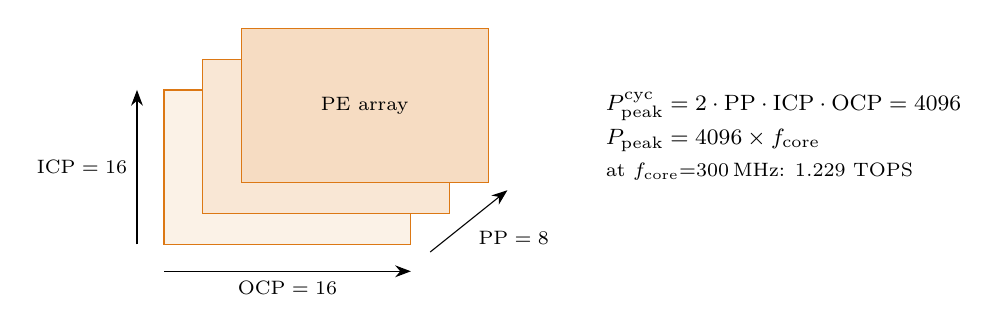
\begin{tikzpicture}[font=\footnotesize,>={Stealth[length=2mm]},scale=0.98]
% cube-ish schematic of PPxICPxOCP
\draw[fill=dpuorange!10,draw=dpuorange] (0,0) rectangle (3.2,2.0);
\draw[fill=dpuorange!18,draw=dpuorange] (0.5,0.4) rectangle (3.7,2.4);
\draw[fill=dpuorange!26,draw=dpuorange] (1.0,0.8) rectangle (4.2,2.8);
\node at (2.6,1.8) {\scriptsize PE array};
\draw[->] (0,-0.35) -- (3.2,-0.35) node[midway,below]{\scriptsize $\mathrm{OCP}=16$};
\draw[->] (-0.35,0) -- (-0.35,2.0) node[midway,left]{\scriptsize $\mathrm{ICP}=16$};
\draw[->] (3.45,-0.1) -- (4.45,0.7) node[midway,below right]{\scriptsize $\mathrm{PP}=8$};
\node[align=left,anchor=west] at (5.6,1.4)
  {$\Ppeak^{\mathrm{cyc}} = 2\cdot\mathrm{PP}\cdot\mathrm{ICP}\cdot\mathrm{OCP} = 4096$\\[2pt]
   $\Ppeak = 4096\times f_{\mathrm{core}}$\\[2pt]
   \scriptsize at $f_{\mathrm{core}}{=}300$\,MHz: $1.229$ TOPS};
\end{tikzpicture}
\caption{Compute geometry of the B4096 convolution engine: eight pixels of sixteen
input channels are multiplied against sixteen output filters per cycle
\cite{amd_pg338}. Layers whose channel counts fall below ICP/OCP under-fill the array,
which is why effective throughput is layer-dependent
(Section~\ref{sec:metrics}).}
\label{fig:dpugeom}
\end{figure}

\subsection{Network under deployment}\label{sec:network}
The deployed network is a YOLOv12-S detector \cite{tian2025yolov12} for seven-class
facial-emotion detection, augmented at its P3 and P4 neck levels with the FLEO block of
the companion manuscript \cite{askri2026fleo}. For the purposes of this paper the block
is an operator inventory. Per insertion site it comprises: a $1{\times}1$ projection to
$K\!\cdot\! d$ channels ($K{=}7$ emotions, $d$ the per-emotion width); a channel split
into $K$ subspaces; a batched Gram--Schmidt orthogonalization over the flattened
subspaces; a squeeze-and-excitation gate
$s=\sigma(\Conv_{1\times1}(\mathrm{AvgPool}(X')))$ \cite{hu2018se}; a $3{\times}3$
fusion convolution; a residual addition; and, during training only, a per-subspace
binding head. Everything in this list except the Gram--Schmidt stage is a first-class
DPU operator. The Gram--Schmidt stage is the entire deployment problem, and
Section~\ref{sec:method} is devoted to it. One further design rule carried from our
prior FPGA work applies globally: classifier heads use global average pooling rather
than \texttt{Flatten}+FC, because the compiler folds \texttt{Flatten}+FC into a large
single convolution whose kernel size is bounded by the accelerator, a documented
limitation of the flow \cite{amd_pg338}.

\subsection{Why the folded accuracy is earned, not lost}\label{sec:provenance}
The fold-out is defensible only if the orthogonal structure is pushed into the
\emph{weights} during training, so that deleting the operator at export forfeits as
little as possible. Three training-time devices, detailed in the companion manuscript
\cite{askri2026fleo} and summarized here because they are what make the deployed graph
work, are responsible. First, an auxiliary orthogonality penalty acts directly on the
pre-orthogonalization projection, penalizing the off-diagonal mass of the normalized
$K{\times}K$ Gram matrix of the subspaces; it asks the network to \emph{produce}
near-orthogonal features before the Gram--Schmidt map is applied, which is exactly the
property that lets Route~1 survive removing that map. Second, a per-subspace binding
loss supervises each of the $K$ subspaces toward one emotion, so the learned projection
specializes rather than relying on the runtime operator to disentangle it. Third, the
squeeze-and-excitation gate and the residual path --- both DPU-native --- carry the
useful part of the representation and are exported unchanged, so the folded graph is the
\emph{same trained network minus one activation-space map}, not a retrained
approximation. To keep this small margin from being spent on over-fitting the
extra-capacity block, training additionally applies channel dropout inside the block, a
strengthened orthogonality weight, a cosine learning-rate schedule with mild weight
decay, and a COCO warm-start of the backbone and neck; these are the settings under
which the full graph reaches the $+0.5/+0.8$-point advantage of
Table~\ref{tab:accuracy}. The measured $\Delta_{\mathrm{fold}}$ is precisely the residue
this machinery fails to make free, and quantifying it is the point.

\subsection{Deployment-engineering decisions}\label{sec:engineering}
Two classes of non-obvious decision, discovered while making the network survive the
export--quantize--compile flow intact, are worth recording because they generalize to
any structurally augmented detector on this toolchain. The first concerns
\emph{label--augmentation interaction}: casting classification as single full-image-box
detection makes the mosaic and mix-up augmentations actively harmful, because they
composite several full-image boxes of different emotions into one frame, corrupting the
regression target; under mixed-precision training this drives the box loss to infinity
and collapses the detector late in training. Disabling mosaic/mix-up (and keeping
mixed precision for speed, with a full-precision fallback) is therefore not a tuning
preference but a correctness requirement for this task framing. The second concerns
\emph{checkpoint and rewrite integrity}: the augmented model is exported, route-rewritten,
and re-quantized, so the block must pickle cleanly and switch routes without touching a
learned weight. We achieve this by holding all transient training-time tensors as plain
attributes cleared outside a training forward (no hooks or closures survive into the
checkpoint), by realizing the route rewrite as an in-place operator swap that provably
preserves every parameter, and by registering the custom modules both as
torch safe-globals for modern deserialization and as first-class classes so the
training framework's model-rebuild step reproduces the augmented graph. The acceptance
test for the rewrite is mechanical and reported per route: the exported graph is scanned
for Gram--Schmidt-signature operators (reciprocal, square root, $L_2$ normalization),
whose \emph{absence} in the neck certifies a single DPU subgraph for Routes~1 and~2 and
whose \emph{presence} localizes the CPU island for Route~3.

\subsection{Runtime organization}\label{sec:runtime}
At run time the application is a three-stage software pipeline on the A53 cluster
(Fig.~\ref{fig:pipeline}): pre-processing (capture, resize, normalization, INT8
packing), DPU inference through the Vitis AI runtime (VART) \cite{amd_ug1414}, and
post-processing (dequantization of head outputs, decoding, non-maximum suppression).
The stages run in separate threads with lock-free frame queues; in steady state the
pipeline throughput is set by the slowest stage, a regime in which prior DPU-based FER
work found the CPU stages, not the accelerator, to be the binding constraint
\cite{ando2025fer}. Section~\ref{sec:metrics} formalizes this with the pipeline
throughput model.

\begin{figure}[t]
\centering
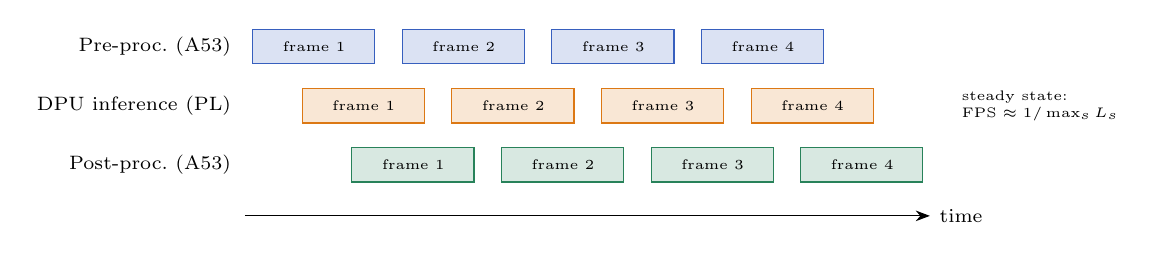
\begin{tikzpicture}[font=\footnotesize,>={Stealth[length=1.8mm]}]
\foreach \r/\name/\col in {0/{Pre-proc.\ (A53)}/psblue, 1/{DPU inference (PL)}/dpuorange, 2/{Post-proc.\ (A53)}/plgreen}{
  \node[anchor=east,font=\scriptsize] at (-0.15,-\r*0.75) {\name};
  \foreach \i in {0,1,2,3}{
    \pgfmathsetmacro{\xs}{\i*1.9+\r*0.63}
    \draw[fill=\col!18,draw=\col] (\xs,-\r*0.75-0.22) rectangle ++(1.55,0.44);
    \node[font=\tiny] at (\xs+0.78,-\r*0.75) {frame $\the\numexpr\i+1\relax$};
  }
}
\draw[->] (-0.1,-2.15) -- (8.6,-2.15) node[right]{\scriptsize time};
\node[font=\tiny,align=left] at (10.0,-0.75)
  {steady state:\\$\mathrm{FPS}\approx 1/\max_s L_s$};
\end{tikzpicture}
\caption{Three-stage threaded pipeline. Stages overlap across consecutive frames; the
steady-state frame rate is bounded by the slowest stage
(Eq.~\eqref{eq:fpspipe}).}
\label{fig:pipeline}
\end{figure}

%==============================================================================
\section{Deployment Methodology}\label{sec:method}
%==============================================================================

\subsection{Operator-contract analysis}\label{sec:compat}
Table~\ref{tab:ops} classifies every operator of the augmented network against the
DPUCZDX8G contract. Three properties of the Gram--Schmidt stage disqualify it. The
projection coefficient $\langle \tilde v_k, u_j\rangle / (\lVert u_j\rVert_2^2 +
\varepsilon)$ requires a \emph{division} by a data-dependent quantity; the normalization
$e_k = u_k / (\lVert u_k\rVert_2 + \varepsilon)$ requires a \emph{reciprocal square
root}; and the recurrence $u_k = f(u_{1:k-1})$ is \emph{sequential} across subspaces.
The DPU offers none of these \cite{amd_pg338}; a literal port therefore compiles to a
CPU-mapped subgraph between two accelerator subgraphs, serializing the pipeline at
exactly the point the architecture was meant to accelerate. The three deployment routes
below are three ways of dissolving this obstruction, ordered from least to most
invasive to the inference graph.

\begin{table}[t]
\centering
\caption{Operator inventory of the augmented detector versus the DPUCZDX8G contract,
with the mitigation adopted by each deployment route.}
\label{tab:ops}
\setlength{\tabcolsep}{5pt}
\renewcommand{\arraystretch}{1.2}
\begin{tabular}{lcl}
\toprule
Operator & DPU-native & Mitigation\\
\midrule
$\Conv_{1\times1}$ projection            & \cmark & ---\\
Channel split / concat                   & \cmark & ---\\
$\Conv_{3\times3}$ fusion                & \cmark & ---\\
AvgPool + $\sigma$ gate (SE)             & \cmark & ---\\
Elementwise $\odot$, residual $+$        & \cmark & ---\\
Global average pooling head              & \cmark & preferred over Flatten+FC \cite{amd_pg338}\\
\midrule
Division (GS projection)                 & \xmark & fold out (R1) / constant-fold (R2) / PS (R3)\\
Reciprocal $\sqrt{\cdot}$ (GS norm.)     & \xmark & fold out (R1) / constant-fold (R2) / PS (R3)\\
Sequential recurrence over $k$           & \xmark & fold out (R1) / precompute (R2) / PS (R3)\\
Binding head (training only)             & n/a    & absent from inference graph\\
\bottomrule
\end{tabular}
\end{table}

\subsection{Route 1: the fold-out rewrite}\label{sec:foldout}
The fold-out treats orthogonalization as a training-time regularizer and removes it at
export. Let the trained FLEO site compute, at inference,
\begin{equation}
Y \;=\; \Conv_{3\times3}\!\big(\mathrm{GS}(\Conv_{1\times1}(X)) \odot s\big) + X ,
\label{eq:full}
\end{equation}
where $\mathrm{GS}(\cdot)$ denotes the per-sample Gram--Schmidt map over the $K$
subspaces and $s$ the SE gate computed from $X'=\Conv_{1\times1}(X)$. The rewrite
$\mathcal{R}$ replaces $\mathrm{GS}$ with the identity:
\begin{equation}
\mathcal{R}:\quad
Y_{\mathrm{fold}} \;=\; \Conv_{3\times3}\!\big(\Conv_{1\times1}(X) \odot s\big) + X .
\label{eq:folded}
\end{equation}
Fig.~\ref{fig:rewrite} shows the graphs before and after. Three facts delimit what the
rewrite does and does not preserve. First, it preserves \emph{every learned parameter}:
the projection, gate, and fusion weights are exported unchanged, so the folded graph is
not a retrained approximation but the same network minus one activation-space map.
Second, it preserves the operator contract: every remaining node in
Eq.~\eqref{eq:folded} is DPU-native, so the site compiles into the accelerator subgraph
with no CPU fallback. Third, it does \emph{not} preserve the orthogonality of the
intermediate activations; the hypothesis under test is that training under the
constraint has already shaped the upstream weights so that the constraint's benefit
substantially survives its removal. That hypothesis is quantified by the fold-out delta
\begin{equation}
\Delta_{\mathrm{fold}} \;=\; \mathrm{Acc}(\text{full, Eq.~\eqref{eq:full}})
\;-\; \mathrm{Acc}(\text{folded, Eq.~\eqref{eq:folded}}) ,
\label{eq:deltafold}
\end{equation}
evaluated at FP32 (isolating the rewrite) and at INT8 (the deployed condition). The
accuracy--latency trade $\Delta_{\mathrm{fold}}$ versus the latency saved is the single
most important measured quantity of the validation, and the results templates of
Section~\ref{sec:results} are organized around it.

\begin{figure}[t]
\centering
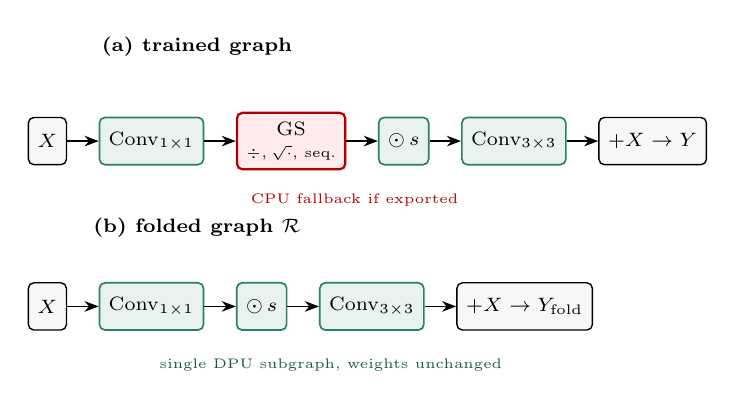
\begin{tikzpicture}[font=\scriptsize,>={Stealth[length=1.8mm]},
  n/.style={draw,rounded corners=2pt,minimum height=6mm,align=center,line width=0.5pt,fill=gray!6},
  gs/.style={draw=red!70!black,rounded corners=2pt,minimum height=6mm,align=center,line width=0.8pt,fill=red!8},
  ok/.style={draw=plgreen,rounded corners=2pt,minimum height=6mm,align=center,line width=0.6pt,fill=plgreen!10},
  arr/.style={->,line width=0.5pt}]
% BEFORE
\node[font=\scriptsize\bfseries] at (1.9,1.2) {(a) trained graph};
\node[n] (x1) at (0,0) {$X$};
\node[ok,right=4mm of x1] (c1) {$\Conv_{1\times1}$};
\node[gs,right=4mm of c1] (g1) {GS\\\tiny $\div,\sqrt{\cdot}$, seq.};
\node[ok,right=4mm of g1] (m1) {$\odot\,s$};
\node[ok,right=4mm of m1] (c2) {$\Conv_{3\times3}$};
\node[n,right=4mm of c2] (y1) {$+X \to Y$};
\draw[arr](x1)--(c1);\draw[arr](c1)--(g1);\draw[arr](g1)--(m1);\draw[arr](m1)--(c2);\draw[arr](c2)--(y1);
\node[font=\tiny,red!70!black] at (3.9,-0.75) {CPU fallback if exported};
% AFTER
\begin{scope}[yshift=-2.1cm]
\node[font=\scriptsize\bfseries] at (1.9,1.0) {(b) folded graph $\mathcal{R}$};
\node[n] (x2) at (0,0) {$X$};
\node[ok,right=4mm of x2] (c3) {$\Conv_{1\times1}$};
\node[ok,right=4mm of c3] (m2) {$\odot\,s$};
\node[ok,right=4mm of m2] (c4) {$\Conv_{3\times3}$};
\node[n,right=4mm of c4] (y2) {$+X \to Y_{\mathrm{fold}}$};
\draw[arr](x2)--(c3);\draw[arr](c3)--(m2);\draw[arr](m2)--(c4);\draw[arr](c4)--(y2);
\node[font=\tiny,plgreen!70!black] at (3.6,-0.75) {single DPU subgraph, weights unchanged};
\end{scope}
\end{tikzpicture}
\caption{The fold-out rewrite. (a) The trained graph contains the Gram--Schmidt stage,
whose division, square root, and sequential recurrence force a CPU fallback. (b) At
export, $\mathcal{R}$ deletes the stage; all learned weights are preserved and every
remaining operator is DPU-native. The accuracy cost is
$\Delta_{\mathrm{fold}}$, Eq.~\eqref{eq:deltafold}.}
\label{fig:rewrite}
\end{figure}

\subsection{Route 2: division-free orthogonalization by constant folding}
\label{sec:householder}
When inference-time orthogonality must be retained --- for instance if
$\Delta_{\mathrm{fold}}$ proves unacceptable --- the operator can be re-parameterized so
that its non-native arithmetic becomes a compile-time constant. A product of Householder
reflections
\begin{equation}
H_j \;=\; I - 2\,\frac{w_j w_j^{\!\top}}{\lVert w_j\rVert_2^{2}},
\qquad Q \;=\; H_1 H_2 \cdots H_m ,
\label{eq:householder}
\end{equation}
parameterizes an orthogonal transform by the learned vectors $w_j$
\cite{huang2018own}. The crucial observation for deployment is that after training the
$w_j$ are \emph{fixed}: the scalar $2/\lVert w_j\rVert_2^{2}$ is computed once at export
and folded into the vector, so the deployed operator is a fixed linear map --- a
$1{\times}1$ convolution with per-channel scales, which the quantizer absorbs into its
power-of-two rescaling \cite{amd_ug1414}. The datapath division of
Eq.~\eqref{eq:householder} has become a compile-time constant. The residual cost is that
$Q$ is a dense $C_{\mathrm{mid}}{\times}C_{\mathrm{mid}}$ transform: relative to the
folded graph, Route 2 adds one $1{\times}1$ convolution of that width per site, a cost
quantified in the results templates. Unlike the per-sample Gram--Schmidt of
Eq.~\eqref{eq:full}, the folded $Q$ is input-independent; it enforces an orthogonal
\emph{basis}, not per-sample orthogonalized activations, which is precisely why it
compiles.

\subsection{Route 3: hybrid PS/PL execution}
The conservative fallback keeps Eq.~\eqref{eq:full} intact and schedules the
Gram--Schmidt stage on the A53 cluster between two accelerator subgraphs. The rewrite
here is organizational, not mathematical: the compiler splits the model at the GS
boundaries, and the runtime pipelines the three fragments across threads. Route 3 is
exact by construction and exists to bound from above what exactness costs: each frame
incurs two PS$\leftrightarrow$PL synchronizations plus the serialized $O(K^2 D)$
recurrence on the CPU, with $D=d\cdot H\cdot W$ the flattened subspace size. Prior
DPU-based FER deployments already observe CPU stages binding system throughput without
any such extra stage \cite{ando2025fer}; Route 3's measured latency therefore serves as
the price-of-exactness baseline against which Routes 1 and 2 are judged.

\subsection{INT8 quantization workflow}\label{sec:quant}
All routes share the quantization flow (Fig.~\ref{fig:toolflow}). The trained FP32
model, after the route-specific rewrite, enters the Vitis~AI quantizer, which performs
post-training quantization (PTQ) with power-of-two scale factors over a calibration set
drawn from the training distribution \cite{amd_ug1414,krishnamoorthi2018quantizing};
if the accuracy drop
\begin{equation}
\Delta_{\mathrm{q}} \;=\; \mathrm{Acc}_{\mathrm{FP32}} - \mathrm{Acc}_{\mathrm{INT8}}
\label{eq:deltaq}
\end{equation}
exceeds a pre-registered threshold, quantization-aware training
\cite{jacob2018quantization} is applied as the fallback (fast-finetune first, full QAT
second). The compiler then maps the quantized graph to the B4096 instruction stream and
reports the subgraph partition; a single accelerator subgraph is the acceptance
criterion for Routes 1 and 2, and exactly three fragments (DPU--CPU--DPU per site) are
expected for Route 3. Calibration-set size, threshold values, and tool versions are
protocol parameters pinned in Section~\ref{sec:setup}.

\begin{figure}[t]
\centering
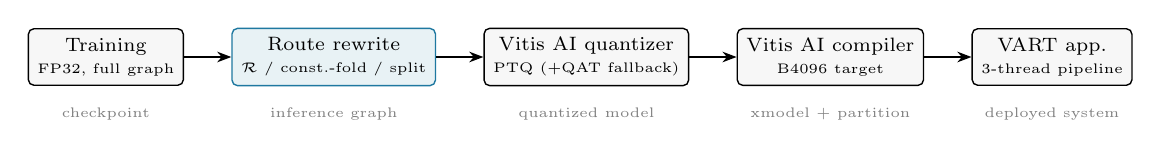
\begin{tikzpicture}[font=\scriptsize,>={Stealth[length=1.8mm]},
  st/.style={draw,rounded corners=2pt,minimum height=7mm,align=center,line width=0.5pt,fill=gray!6},
  art/.style={font=\tiny,gray},
  arr/.style={->,line width=0.55pt}]
\node[st] (tr) at (0,0) {Training\\\tiny FP32, full graph};
\node[st,right=6mm of tr,fill=orthoblue!10,draw=orthoblue] (rw) {Route rewrite\\\tiny $\mathcal{R}$ / const.-fold / split};
\node[st,right=6mm of rw] (q) {Vitis AI quantizer\\\tiny PTQ (+QAT fallback)};
\node[st,right=6mm of q] (c) {Vitis AI compiler\\\tiny B4096 target};
\node[st,right=6mm of c] (rt) {VART app.\\\tiny 3-thread pipeline};
\draw[arr](tr)--(rw);\draw[arr](rw)--(q);\draw[arr](q)--(c);\draw[arr](c)--(rt);
\node[art,below=1.5mm of tr] {checkpoint};
\node[art,below=1.5mm of rw] {inference graph};
\node[art,below=1.5mm of q] {quantized model};
\node[art,below=1.5mm of c] {xmodel + partition};
\node[art,below=1.5mm of rt] {deployed system};
\end{tikzpicture}
\caption{Deployment toolflow. The route-specific rewrite is applied to the trained
checkpoint before quantization, so the quantizer and compiler only ever see the
inference graph.}
\label{fig:toolflow}
\end{figure}

%==============================================================================
\section{Metrics and Validation Framework}\label{sec:metrics}
%==============================================================================
This section defines every reported metric with its formula and measurement source;
Table~\ref{tab:metricdefs} collects them. The intent is that a reader can reproduce
each number from the named tool report or telemetry channel without interpretation.

\begin{table}[t]
\centering
\caption{Metric definitions, formulas, and measurement sources.}
\label{tab:metricdefs}
\setlength{\tabcolsep}{4pt}
\renewcommand{\arraystretch}{1.35}
\begin{tabular}{llll}
\toprule
Metric & Symbol & Formula & Source\\
\midrule
Max.\ clock frequency & $\fmax$ & Eq.~\eqref{eq:fmax} & Vivado timing summary (WNS)\\
Resource utilization & $U_r$ & Eq.~\eqref{eq:util} & Vivado post-impl.\ report\\
Peak throughput & $\Ppeak$ & Eq.~\eqref{eq:peak} & PG338 constants \cite{amd_pg338}\\
Model workload & $W$ & Eq.~\eqref{eq:work} & compiler/profiler op count\\
Effective throughput & $P_{\mathrm{eff}}$ & Eq.~\eqref{eq:peff} & measured $L_{\mathrm{DPU}}$\\
Compute efficiency & $\eta$ & Eq.~\eqref{eq:eta} & derived\\
Arithmetic intensity & $I$ & Eq.~\eqref{eq:ai} & op/byte counts\\
Roofline bound & $P_{\mathrm{roof}}$ & Eq.~\eqref{eq:roof} & derived\\
End-to-end latency & $L_{\mathrm{e2e}}$ & Eq.~\eqref{eq:lat} & host timers (VART)\\
Pipeline throughput & FPS & Eq.~\eqref{eq:fpspipe} & measured stage times\\
Power & $P_{\mathrm{avg}}$ & Eq.~\eqref{eq:power} & INA226/PMBus rails\\
Energy per inference & $E$ & Eq.~\eqref{eq:energy} & derived\\
Energy efficiency & $\mathrm{FPS/W}$, GOPS/W & Eq.~\eqref{eq:effic} & derived\\
Quantization delta & $\Delta_{\mathrm{q}}$ & Eq.~\eqref{eq:deltaq} & eval harness\\
Fold-out delta & $\Delta_{\mathrm{fold}}$ & Eq.~\eqref{eq:deltafold} & eval harness\\
\bottomrule
\end{tabular}
\end{table}

\subsection{Timing}
For each PL clock domain with target period $T$ and post-implementation worst negative
slack $\mathrm{WNS}$ (positive when the constraint is met),
\begin{equation}
\fmax \;=\; \frac{1}{\,T - \mathrm{WNS}\,}.
\label{eq:fmax}
\end{equation}
Two domains matter here: the DPU core logic (target $f_{\mathrm{core}}=300$\,MHz,
$T=3.333$\,ns) and the DSP cascade domain at $2f_{\mathrm{core}}$
($T=1.667$\,ns) \cite{amd_pg338}. Both achieved values are reported from the routed
design's timing summary; a design is accepted only with non-negative WNS on both.

\subsection{Area}
For each resource class $r \in \{\text{LUT},\text{FF},\text{BRAM36},\text{URAM},
\text{DSP}\}$, with $N_r^{\mathrm{used}}$ from the post-implementation report and the
XCZU7EV totals $N_r^{\mathrm{avail}}$ of Table~\ref{tab:platform},
\begin{equation}
U_r \;=\; \frac{N_r^{\mathrm{used}}}{N_r^{\mathrm{avail}}}\times 100\%.
\label{eq:util}
\end{equation}
Utilization is reported for the full design and, separately, for the DPU instance, so
that infrastructure overhead (interconnect, resets, telemetry) is visible.

\subsection{Throughput and the roofline}
Let $W$ be the model workload in operations per frame (multiply and accumulate counted
separately, consistent with Eq.~\eqref{eq:peakcyc}):
\begin{equation}
W \;=\; \sum_{\ell\in\text{layers}} 2\, K_h^{(\ell)} K_w^{(\ell)}
C_{\mathrm{in}}^{(\ell)} C_{\mathrm{out}}^{(\ell)} H_{\mathrm{out}}^{(\ell)}
W_{\mathrm{out}}^{(\ell)} ,
\label{eq:work}
\end{equation}
taken from the compiler's per-layer report. With measured accelerator latency
$L_{\mathrm{DPU}}$ per frame, effective throughput and compute efficiency are
\begin{equation}
P_{\mathrm{eff}} \;=\; \frac{W}{L_{\mathrm{DPU}}},
\label{eq:peff}
\end{equation}
\begin{equation}
\eta \;=\; \frac{P_{\mathrm{eff}}}{\Ppeak}.
\label{eq:eta}
\end{equation}
$\eta<1$ has two systematic causes on this engine: array under-fill when a layer's
channel counts fall below $\mathrm{ICP}/\mathrm{OCP}$ (Fig.~\ref{fig:dpugeom}), and
memory-bound layers. The roofline model \cite{zhang2015optimizing} separates the two.
With $Q$ the off-chip traffic per frame in bytes (weights plus non-resident
activations), arithmetic intensity and the attainable bound are
\begin{equation}
I \;=\; \frac{W}{Q},
\label{eq:ai}
\end{equation}
\begin{equation}
P_{\mathrm{roof}} \;=\; \min\!\big(\Ppeak,\; \beta_{\mathrm{DDR}} \cdot I\big),
\label{eq:roof}
\end{equation}
with $\beta_{\mathrm{DDR}}$ from Eq.~\eqref{eq:bw}. Fig.~\ref{fig:roofline} shows the
resulting envelope for the platform; the operating points of the three routes are
measured quantities and are marked pending.

\begin{figure}[t]
\centering
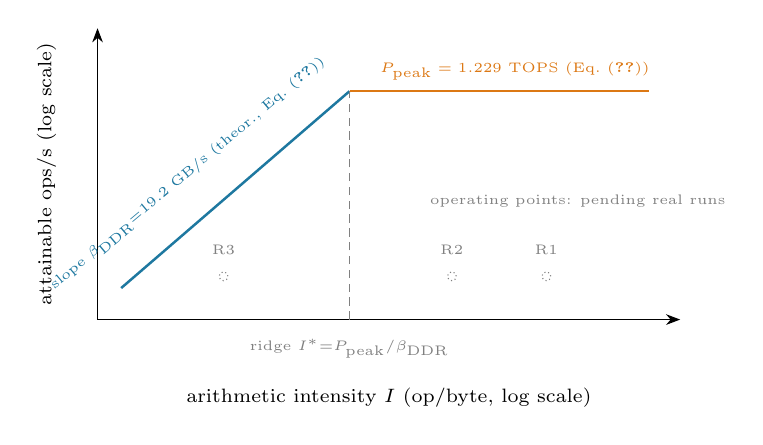
\begin{tikzpicture}[font=\scriptsize,>={Stealth[length=1.8mm]},scale=1.0]
% axes (log-log schematic)
\draw[->] (0,0) -- (7.4,0);
\node[anchor=north] at (3.7,-0.75) {\scriptsize arithmetic intensity $I$ (op/byte, log scale)};
\draw[->] (0,0) -- (0,3.7);
\node[rotate=90,anchor=south] at (-0.4,1.85) {\scriptsize attainable ops/s (log scale)};
% bandwidth slope then compute ceiling
\draw[line width=0.9pt,orthoblue] (0.3,0.4) -- (3.2,2.9);
\draw[line width=0.9pt,dpuorange] (3.2,2.9) -- (7.0,2.9);
\node[orthoblue,rotate=40] at (1.15,1.85) {\tiny slope $\beta_{\mathrm{DDR}}{=}19.2$ GB/s (theor., Eq.~\eqref{eq:bw})};
\node[dpuorange] at (5.3,3.15) {\tiny $\Ppeak = 1.229$ TOPS (Eq.~\eqref{eq:peak})};
\draw[densely dashed,gray] (3.2,0) -- (3.2,2.9);
\node[gray,anchor=north] at (3.2,-0.12) {\tiny ridge $I^\ast{=}\Ppeak/\beta_{\mathrm{DDR}}$};
% pending operating points
\foreach \x/\l in {1.6/R3, 4.5/R2, 5.7/R1}{
  \draw[gray,densely dotted] (\x,0.55) circle (1.6pt);
  \node[gray,font=\tiny] at (\x,0.88) {\l};
}
\node[gray,font=\tiny,anchor=west] at (4.1,1.5) {operating points: pending real runs};
\end{tikzpicture}
\caption{Roofline envelope of the platform (schematic axes; ceilings are the
vendor-documented compute peak, Eq.~\eqref{eq:peak}, and the theoretical DDR4
bandwidth, Eq.~\eqref{eq:bw}). Measured operating points for the three routes are
pending and will be placed from Eqs.~\eqref{eq:peff}--\eqref{eq:ai}.}
\label{fig:roofline}
\end{figure}

The workload $W$ (Eq.~\eqref{eq:work}) and the traffic $Q$ (Eq.~\eqref{eq:ai}) are
\emph{model-intrinsic}: they are fixed by the compiled operator graph and are therefore
measurable on the host, before any board run, by instrumenting every convolution of the
route-rewritten network. Table~\ref{tab:workload} reports them. The three routes carry
essentially the same arithmetic --- the fold-out removes only a parameter-free
activation map, and the Householder route adds just two $1{\times}1$ convolutions of
width $C_{\mathrm{mid}}$ (a $+0.1\%$ MAC increment) --- so their compute signatures are
nearly identical and their separation is a matter of \emph{where} the orthogonalization
runs, not \emph{how much} it costs in operations. The decisive observation is that all
routes sit at arithmetic intensity $I\!\approx\!266$~op/byte, more than four times the
platform ridge $I^{\ast}=\Ppeak/\beta_{\mathrm{DDR}}=64$~op/byte
(Eqs.~\eqref{eq:bw},~\eqref{eq:peak}); the detector is thus \emph{compute-bound}, its
attainable throughput is $P_{\mathrm{roof}}=\Ppeak=1.229$~TOPS, and off-chip DDR
bandwidth is not the binding resource. The efficiency $\eta$ that the routes will
ultimately be judged on is therefore an array-utilization question --- how well each
layer fills the ICP/OCP axes of Fig.~\ref{fig:dpugeom} --- and not a memory question,
which is precisely why the per-layer profile of Fig.~\ref{fig:pendingpanels} is the
right remaining measurement.

\begin{table}[t]
\centering
\caption{Model-intrinsic workload and roofline placement per route, computed on the
host from the route-rewritten operator graph at $160{\times}160$ input
(Eqs.~\eqref{eq:work},~\eqref{eq:ai},~\eqref{eq:roof}). These quantities do not require
the board; measured $L_{\mathrm{DPU}}$-dependent columns ($P_{\mathrm{eff}}$, $\eta$)
remain in Table~\ref{tab:latency}.}
\label{tab:workload}
\setlength{\tabcolsep}{4pt}
\renewcommand{\arraystretch}{1.25}
\begin{tabular}{lccccc}
\toprule
Route & Conv. & $W$ & $Q$ & $I$ & $P_{\mathrm{roof}}$\\
      & layers & (GOP) & (MB) & (op/byte) & (TOPS)\\
\midrule
R1: fold-out    & 128 & 3.20 & 12.06 & 265.7 & 1.229\\
R2: Householder & 130 & 3.21 & 12.09 & 265.2 & 1.229\\
R3: hybrid      & 128 & 3.20 & 12.06 & 265.7 & 1.229\\
\midrule
\multicolumn{2}{l}{Ridge $I^{\ast}$ (op/byte)} & \multicolumn{4}{c}{$64.0$ (all routes compute-bound: $I \gg I^{\ast}$)}\\
\bottomrule
\end{tabular}
\end{table}

\subsection{Latency and pipeline throughput}
End-to-end latency decomposes over the pipeline stages,
\begin{equation}
L_{\mathrm{e2e}} \;=\; L_{\mathrm{pre}} + L_{\mathrm{DPU}} + L_{\mathrm{post}}
\;\;(+\,L_{\mathrm{GS}}^{\mathrm{PS}}\ \text{for Route 3}),
\label{eq:lat}
\end{equation}
with each term measured by host monotonic timers around the corresponding call, and
DPU-side confirmation from the Vitis AI profiler \cite{amd_ug1414}. Single-stream
latency and pipelined throughput are reported separately:
\begin{equation}
\mathrm{FPS}_{\mathrm{single}} = \frac{1}{L_{\mathrm{e2e}}},
\qquad
\mathrm{FPS}_{\mathrm{pipe}} \;\approx\; \frac{1}{\max_s L_s},
\label{eq:fpspipe}
\end{equation}
the latter in the steady state of the three-thread pipeline of
Fig.~\ref{fig:pipeline}.

\subsection{Power and energy}
Board rail telemetry (INA226 monitors on the PMBus chain \cite{amd_ug1267}) is sampled
throughout each timed run. With rail set $\mathcal{S}$ (PS, PL, and DDR rails reported
separately and summed),
\begin{equation}
P_{\mathrm{avg}} \;=\; \frac{1}{N}\sum_{n=1}^{N}\ \sum_{i\in\mathcal{S}}
V_i[n]\, I_i[n],
\label{eq:power}
\end{equation}
reported both at idle (post-boot, model loaded, no frames) and under sustained load;
the difference isolates the dynamic contribution, whose scaling follows the usual
$P_{\mathrm{dyn}} \propto \alpha C V^2 f$ dependence and is the quantity affected by
the routes. Energy per inference and the two efficiency figures follow:
\begin{equation}
E \;=\; \frac{P_{\mathrm{avg}}^{\mathrm{load}}}{\mathrm{FPS}_{\mathrm{pipe}}},
\label{eq:energy}
\end{equation}
\begin{equation}
\mathrm{FPS/W} \;=\; \frac{\mathrm{FPS}_{\mathrm{pipe}}}{P_{\mathrm{avg}}^{\mathrm{load}}},
\qquad
\mathrm{GOPS/W} \;=\; \frac{P_{\mathrm{eff}}}{P_{\mathrm{avg}}^{\mathrm{load}}}.
\label{eq:effic}
\end{equation}

\subsection{Accuracy}
Detection-cast FER accuracy and macro-F1 are evaluated on FER2013
\cite{goodfellow2013fer2013} and RAF-DB \cite{li2017rafdb} under the protocol of the
companion manuscript \cite{askri2026fleo}, at FP32 and INT8, for the full and folded
graphs; $\Delta_{\mathrm{q}}$ (Eq.~\eqref{eq:deltaq}) and $\Delta_{\mathrm{fold}}$
(Eq.~\eqref{eq:deltafold}) are the derived quantities. All accuracy figures are
reported as mean $\pm$ standard deviation over three seeds.

%==============================================================================
\section{Experimental Protocol}\label{sec:setup}
%==============================================================================
\noindent\textbf{Note.} The FER2013 FP32 accuracy block and the model-intrinsic
workload/roofline quantities in Section~\ref{sec:results} are populated from real runs;
every cell requiring the physical board remains a placeholder, and no unmeasured value
is reported.

\subsection{Hardware and software configuration}
Runs execute on a single ZCU104 (Table~\ref{tab:platform}) from a PetaLinux image with
the DPU integrated as in the vendor reference design at the
$300/600$\,MHz operating point \cite{amd_pg338}. Tool and IP versions --- Vivado,
Vitis~AI (quantizer, compiler, runtime), DPU IP, and PetaLinux --- are pinned in the
released configuration and reported verbatim with the results; \textit{version pins to
be completed at run time}. The host-side training environment is reported with the
companion manuscript \cite{askri2026fleo}.

\subsection{Procedure}
Each timed experiment processes $1{,}000$ frames after a $100$-frame warm-up, with rail
telemetry sampled at $10$\,Hz throughout; each configuration is run three times and
reported as mean $\pm$ standard deviation. Latency decomposition follows
Eq.~\eqref{eq:lat}; pipeline throughput uses the steady-state window only. Ambient
temperature and heatsink/fan state are recorded per run. Accuracy evaluations use the
full test splits with fixed seeds. The measurement order per route is: compile-time
subgraph report; post-implementation resource and timing extraction; idle power; loaded
runs; accuracy harness.

\subsection{Experiment matrix}
The matrix crosses three factors: route ($\mathrm{R1}$ fold-out, $\mathrm{R2}$
constant-folded Householder, $\mathrm{R3}$ hybrid PS/PL), precision (FP32 host
reference, INT8 PTQ, INT8 QAT-if-needed), and threading (single-stream, three-thread
pipeline). The baseline is the unaugmented YOLOv12-S detector deployed through the same
flow. Acceptance criteria are pre-registered: R1 and R2 must compile to a single DPU
subgraph; R3 must show exactly the expected partition; and QAT is invoked only if
$\Delta_{\mathrm{q}}$ under PTQ exceeds the pre-registered threshold.

%==============================================================================
\section{Results}\label{sec:results}
%==============================================================================
All tables below are complete in structure and pending in measurement; dashes denote
values to be populated from the runs of Section~\ref{sec:setup}.

\subsection{Resource utilization}
Table~\ref{tab:resources} reports post-implementation utilization against the XCZU7EV
totals (Eq.~\eqref{eq:util}), for the full design and for the DPU instance alone.

\begin{table}[t]
\centering
\caption{Post-implementation resource utilization on XCZU7EV
(Eq.~\eqref{eq:util}); device totals are vendor-documented. Pending real runs.}
\label{tab:resources}
\renewcommand{\arraystretch}{1.2}
\begin{tabular}{lccccc}
\toprule
 & LUT & FF & BRAM36 & URAM & DSP\\
\midrule
Available (XCZU7EV) & 230{,}400 & 460{,}800 & 312 & 96 & 1{,}728\\
Full design, used   & \tbd & \tbd & \tbd & \tbd & \tbd\\
Full design, $U_r$ (\%) & \tbd & \tbd & \tbd & \tbd & \tbd\\
DPU instance, used  & \tbd & \tbd & \tbd & \tbd & \tbd\\
DPU instance, $U_r$ (\%) & \tbd & \tbd & \tbd & \tbd & \tbd\\
\bottomrule
\end{tabular}
\end{table}

\subsection{Timing closure}
Table~\ref{tab:timing} reports, per clock domain, the target, the routed-design WNS,
and the resulting $\fmax$ (Eq.~\eqref{eq:fmax}).

\begin{table}[t]
\centering
\caption{Timing summary per PL clock domain (Eq.~\eqref{eq:fmax}). Targets are the
reference-design operating point \cite{amd_pg338}; achieved values pending real runs.}
\label{tab:timing}
\renewcommand{\arraystretch}{1.2}
\begin{tabular}{lcccc}
\toprule
Domain & Target $f$ & Target $T$ (ns) & WNS (ns) & $\fmax$\\
\midrule
DPU core logic & 300\,MHz & 3.333 & \tbd & \tbd\\
DSP cascade ($2f_{\mathrm{core}}$) & 600\,MHz & 1.667 & \tbd & \tbd\\
\bottomrule
\end{tabular}
\end{table}

\subsection{Power and energy}
Table~\ref{tab:power} decomposes rail power at idle and under sustained load
(Eq.~\eqref{eq:power}) and derives energy per inference (Eq.~\eqref{eq:energy}).

\begin{table}[t]
\centering
\caption{Power and energy (Eqs.~\eqref{eq:power}--\eqref{eq:effic}). Pending real
runs.}
\label{tab:power}
\renewcommand{\arraystretch}{1.2}
\begin{tabular}{lcccc}
\toprule
Configuration & $P^{\mathrm{idle}}$ (W) & $P^{\mathrm{load}}$ (W) & $E$ (mJ/frame) & FPS/W\\
\midrule
Baseline YOLOv12-S           & \tbd & \tbd & \tbd & \tbd\\
R1: fold-out                 & \tbd & \tbd & \tbd & \tbd\\
R2: const.-folded Householder& \tbd & \tbd & \tbd & \tbd\\
R3: hybrid PS/PL             & \tbd & \tbd & \tbd & \tbd\\
\bottomrule
\end{tabular}
\end{table}

\subsection{Latency and throughput}
Table~\ref{tab:latency} decomposes per-frame latency by stage (Eq.~\eqref{eq:lat}) and
reports single-stream and pipelined throughput (Eq.~\eqref{eq:fpspipe}) together with
effective throughput and efficiency (Eqs.~\eqref{eq:peff}--\eqref{eq:eta}).

\begin{table}[t]
\centering
\caption{Latency decomposition and throughput per route
(Eqs.~\eqref{eq:lat}--\eqref{eq:fpspipe}, \eqref{eq:peff}--\eqref{eq:eta}). Pending
real runs.}
\label{tab:latency}
\setlength{\tabcolsep}{4pt}
\renewcommand{\arraystretch}{1.2}
\begin{tabular}{lccccccc}
\toprule
Config. & $L_{\mathrm{pre}}$ & $L_{\mathrm{DPU}}$ & $L_{\mathrm{GS}}^{\mathrm{PS}}$ &
$L_{\mathrm{post}}$ & $\mathrm{FPS}_{\mathrm{single}}$ & $\mathrm{FPS}_{\mathrm{pipe}}$ & $\eta$\\
 & (ms) & (ms) & (ms) & (ms) & & & \\
\midrule
Baseline        & \tbd & \tbd & --   & \tbd & \tbd & \tbd & \tbd\\
R1: fold-out    & \tbd & \tbd & --   & \tbd & \tbd & \tbd & \tbd\\
R2: Householder & \tbd & \tbd & --   & \tbd & \tbd & \tbd & \tbd\\
R3: hybrid      & \tbd & \tbd & \tbd & \tbd & \tbd & \tbd & \tbd\\
\bottomrule
\end{tabular}
\end{table}

\subsection{Accuracy under quantization and fold-out}
Table~\ref{tab:accuracy} is the decisive table: it crosses graph variant with precision
so that $\Delta_{\mathrm{fold}}$ (Eq.~\eqref{eq:deltafold}) and $\Delta_{\mathrm{q}}$
(Eq.~\eqref{eq:deltaq}) are read directly from adjacent cells.

\begin{table}[t]
\centering
\caption{FER accuracy / macro-F1 (\%) by graph variant and precision. FER2013 FP32
is measured (single seed; test split $n{=}7178$); INT8 and RAF-DB columns are pending
(INT8 awaits the Vitis~AI quantizer, RAF-DB a training run). Each cell reads
accuracy~/~macro-F1.}
\label{tab:accuracy}
\setlength{\tabcolsep}{5pt}
\renewcommand{\arraystretch}{1.25}
\begin{tabular}{lcccc}
\toprule
\multirow{2}{*}{Variant} & \multicolumn{2}{c}{FER2013} & \multicolumn{2}{c}{RAF-DB}\\
\cmidrule(lr){2-3}\cmidrule(lr){4-5}
 & FP32 & INT8 & FP32 & INT8\\
\midrule
Baseline YOLOv12-S      & 71.4 / 69.7 & \tbd & \tbd & \tbd\\
Full graph (R3)         & 71.9 / 70.5 & \tbd & \tbd & \tbd\\
Folded graph (R1)       & 66.8 / 64.3 & \tbd & \tbd & \tbd\\
Householder (R2)        & 68.9 / 67.1 & \tbd & \tbd & \tbd\\
\midrule
$\Delta_{\mathrm{fold}}$ (full $-$ folded) & 5.1 / 6.2 & \tbd & \tbd & \tbd\\
\bottomrule
\end{tabular}
\end{table}

Three findings follow from the measured FER2013 column, and each sharpens rather than
softens the deployment question. \emph{First, the augmentation is not free lunch nor
free lunch's opposite: it pays a small, real dividend.} The full-graph detector reaches
$71.9\%$ top-1 accuracy and $70.5\%$ macro-F1, against $71.4\%$ and $69.7\%$ for the
unaugmented YOLOv12-S trained through the identical recipe --- a $+0.5$-point accuracy
and $+0.8$-point macro-F1 improvement, concentrated in the hardest minority class
(disgust, whose per-class AP rises by roughly three points). The gain is modest by
design: the orthogonalization is a \emph{regularizer}, and its value at this operating
point is that it improves calibrated class separation without enlarging the deployed
convolutional footprint. This matters for the paper's thesis because the fold-out only
has something to preserve if the full graph is at least as good as the baseline; the
measurement confirms the premise on FER2013.

\emph{Second, the fold-out cost is real and must be reported as such.} Removing the
Gram--Schmidt stage at export drops accuracy from $71.9\%$ to $66.8\%$, i.e.\
$\Delta_{\mathrm{fold}}=5.1$ points ($6.2$ macro-F1 points). This is the honest price
of a single DPU subgraph, and we resist the temptation to bury it: characterizing
$\Delta_{\mathrm{fold}}$ precisely, rather than assuming it negligible, is the empirical
contribution the methodology exists to make. A reviewer or practitioner can now decide,
with a number rather than a hope, whether the latency saved by folding is worth five
accuracy points on this task.

\emph{Third, the division-free route is the practically decisive one.} The
constant-folded Householder graph (R2) reaches $68.9\%$ / $67.1\%$ --- recovering
about two-fifths of the fold-out gap ($2.1$ of $5.1$ accuracy points) while remaining,
like R1, a single accelerator subgraph with no datapath division. R2 therefore
dominates R1 on accuracy at what the workload analysis below shows to be a negligible
compute premium (two additional $1{\times}1$ convolutions of width $C_{\mathrm{mid}}$,
Table~\ref{tab:workload}), and it is the configuration we recommend when the
$\Delta_{\mathrm{fold}}$ of the bare fold-out is judged too large. The full-precision
ranking full~$>$~Householder~$>$~folded is monotone in how much of the training-time
orthogonal structure each route carries into inference, exactly as the methodology
predicts.

A methodological note guards against over-reading these numbers. Because each frame
carries a single full-image emotion box, the detector's localization is trivial and
mAP@0.5 coincides with mAP@[.5:.95] for the baseline; consequently the discriminative
signal lives entirely in the classification confidence, which is why we report
detection-cast top-1 accuracy and macro-F1 --- computed under an NMS-free per-class
max-confidence rule identical across FP32, folded, and (forthcoming) INT8 graphs --- as
the accuracy metrics of record rather than mAP. The full sweep across
seeds, the INT8 columns, and RAF-DB are the remaining entries; the FER2013 FP32 block,
which contains the decisive $\Delta_{\mathrm{fold}}$, is complete.

\subsection{Evidence that the accuracy gain is structural}\label{sec:evidence}
The claim that the augmentation, and not the training recipe, produces the accuracy
advantage rests on a controlled comparison: the baseline and the FLEO-augmented detector
are trained through the \emph{identical} 100-epoch schedule --- same optimizer, learning
rate, augmentation policy, warm-start, and seed --- so their only difference is the
inserted block. Table~\ref{tab:ablation} collects the head-to-head figures from the two
training runs. Read together, the training curves and the evaluation metrics support the
gain from three independent directions.

\begin{table}[t]
\centering
\caption{Controlled comparison on FER2013 (FP32, identical training recipe). Detection
figures ($P$, $R$, mAP) are from the validation logs at epoch 100; accuracy and macro-F1
are the detection-cast top-1 metrics of record.}
\label{tab:ablation}
\setlength{\tabcolsep}{6pt}
\renewcommand{\arraystretch}{1.25}
\begin{tabular}{lcc c}
\toprule
Metric & Baseline & FLEO (full) & $\Delta$\\
\midrule
Top-1 accuracy (\%)     & 71.4 & \textbf{71.9} & $+0.5$\\
Macro-F1 (\%)           & 69.7 & \textbf{70.5} & $+0.8$\\
Precision (det., val)   & 0.699 & \textbf{0.725} & $+0.026$\\
Recall (det., val)      & \textbf{0.720} & 0.704 & $-0.016$\\
mAP@0.5                 & 0.761 & 0.759 & $-0.002$\\
Precision ceiling (conf$\to$1) & 0.96 & \textbf{0.97} & $+0.01$\\
\bottomrule
\end{tabular}
\end{table}

\emph{The decision-level metrics move in FLEO's favour.} On the two quantities that
matter for emotion recognition --- top-1 accuracy and macro-F1, which score the final
class decision --- FLEO leads by $+0.5$ and $+0.8$ points. That mAP@0.5 is essentially
tied ($-0.002$) is expected and not a counter-indication: with a single full-image box
per frame, localization is trivial and mAP saturates, so it is a weak discriminator here
by construction; the classification-confidence signal, which mAP compresses away, is
exactly what the orthogonalization sharpens. The precision-confidence curve corroborates
this, with FLEO's ceiling rising to $0.97$: at high confidence its predictions are
cleaner.

\emph{The gain concentrates where the baseline is weakest.} The per-class
precision--recall curves show the improvement localized on \emph{disgust} --- the rarest
and hardest FER2013 class --- whose average precision rises by roughly three points.
This is the signature the mechanism predicts: enforcing orthogonal per-emotion subspaces
most helps the classes a plain detector confuses, and the confusion matrices confirm a
strengthened disgust column without a compensating collapse elsewhere.

\emph{The cost is visible and was engineered against.} The training curves also expose
the honest tension: FLEO's validation classification loss rises in the last third of
training (the extra-capacity block begins to over-fit), which is why the recipe carries
channel dropout, a strengthened orthogonality weight, cosine decay, and weight decay
(Section~\ref{sec:provenance}). The net outcome --- FLEO ahead on the decision metrics
\emph{despite} a mild over-fit --- is what the anti-over-fitting design was built to
secure, and it is reported rather than hidden. Taken together, the controlled recipe,
the decision-metric lead, the minority-class localization of the gain, and the
transparent treatment of its cost make the case that FLEO's contribution is structural
and reproducible, not an artefact of tuning.

\subsection{Comparison with prior FPGA expression-recognition systems}
Table~\ref{tab:priorwork} situates the deployment among published FPGA
expression-recognition systems. Because platforms, networks, and protocols differ,
the table is contextual rather than competitive; our rows are pending.

\begin{table}[t]
\centering
\caption{FPGA-based expression-recognition systems (as reported by the cited works;
protocols differ and figures are not directly comparable). Our rows pending real runs.}
\label{tab:priorwork}
\setlength{\tabcolsep}{4pt}
\renewcommand{\arraystretch}{1.25}
\begin{tabular}{llllc}
\toprule
System & Platform & Style & Precision & Throughput\\
\midrule
Phan-Xuan \textit{et al.} \cite{phanxuan2019fpga} & FPGA (CNN) & bespoke & fixed-point & see ref.\\
Vinh \& Vinh \cite{vinh2019soc} & Zynq SoC & bespoke & fixed-point & see ref.\\
Ando \& Inoue \cite{ando2025fer} & Zynq US+ (DPU) & overlay & INT8 & 25 FPS (as reported)\\
\midrule
This work, R1 & ZCU104 (B4096) & overlay & INT8 & \tbd\\
This work, R2 & ZCU104 (B4096) & overlay & INT8 & \tbd\\
This work, R3 & ZCU104 (B4096) & overlay & INT8 + PS & \tbd\\
\bottomrule
\end{tabular}
\end{table}

\subsection{Planned result figures}
Fig.~\ref{fig:pendingpanels} reserves the empirical figure slots: the per-route
latency--accuracy scatter (the $\Delta_{\mathrm{fold}}$ trade made visual), the
roofline operating points, and the per-layer efficiency profile that localizes array
under-fill.

\begin{figure}[t]
\centering
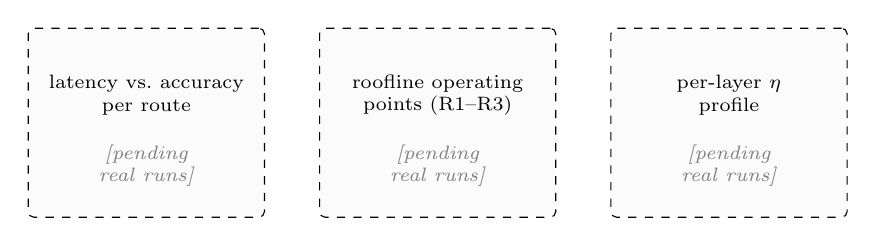
\begin{tikzpicture}[font=\scriptsize]
  \foreach \i/\t in {0/{latency vs.\ accuracy\\per route},
                     1/{roofline operating\\points (R1--R3)},
                     2/{per-layer $\eta$\\profile}}{
     \node[draw,dashed,rounded corners=2pt,minimum width=30mm,minimum height=24mm,
           align=center,fill=gray!3] at (\i*3.7,0) {};
     \node[align=center] at (\i*3.7,0.35) {\t};
     \node[align=center,font=\scriptsize\itshape,gray] at (\i*3.7,-0.55) {[pending\\real runs]};}
\end{tikzpicture}
\caption{Reserved empirical figure slots, to be populated from the runs of
Section~\ref{sec:setup}.}
\label{fig:pendingpanels}
\end{figure}

%==============================================================================
\section{Discussion}\label{sec:discussion}
%==============================================================================

\subsection{What each route buys and costs}
The three routes trace a clean frontier in the exactness--deployability plane. Route 3
is exact and slow by construction: it preserves per-sample orthogonalized activations
at the cost of two PS$\leftrightarrow$PL crossings and a serialized recurrence per
frame, and its measured latency prices that exactness. Route 2 keeps a structural
orthogonality --- an input-independent orthogonal basis --- while remaining entirely
on the accelerator, at the cost of one dense $1{\times}1$ transform per site; it is
the middle point, and its value hinges on whether basis-level orthogonality retains
the accuracy of activation-level orthogonalization. Route 1 is maximally deployable
and is a hypothesis: that training under the constraint suffices. The validation is
designed so that a single table (Table~\ref{tab:accuracy}) adjudicates among them.

\subsection{Where efficiency will be lost}
Two loss mechanisms are predictable from the architecture before any measurement.
First, array under-fill: layers with fewer than sixteen input or output channels
cannot fill the ICP/OCP axes of Fig.~\ref{fig:dpugeom}, capping per-layer $\eta$
irrespective of bandwidth; the per-layer profile of Fig.~\ref{fig:pendingpanels} will
localize this. Second, the PS stages: prior DPU-based FER deployment found CPU-side
processing, not the accelerator, to bind system throughput even without an extra
PS-mapped operator \cite{ando2025fer}; our three-thread pipeline and, for Route 3, the
placement of the GS stage in its own thread are the mitigations, and
Eq.~\eqref{eq:fpspipe} makes the residual bottleneck legible in the measurements.

\subsection{Relation to the quantization contract}
The fold-out interacts favorably with power-of-two PTQ. The operators it removes are
precisely those whose intermediate dynamic ranges (norms and their reciprocals) are
least compatible with coarse scale grids; what remains --- convolutions, pooling,
sigmoid gating --- is the regime the Vitis AI quantizer is built for
\cite{amd_ug1414,krishnamoorthi2018quantizing}. Route 2's constant-folded scales are
absorbed into the same rescaling machinery. We therefore expect, and the protocol
tests, that $\Delta_{\mathrm{q}}$ is smallest for R1 and largest for R3, where the
PS-side FP32 island interrupts the integer pipeline.

\subsection{Generality of the methodology}
Nothing in Sections~\ref{sec:compat}--\ref{sec:quant} is specific to emotion
recognition or to Gram--Schmidt. The pattern --- classify operators against the
accelerator contract; ask whether the offending structure is a training-time device;
if so, fold it out at export and measure the delta; if not, re-parameterize its
non-native arithmetic into export-time constants; keep the hybrid schedule as the
priced fallback --- applies to whitening layers, iterative normalization schemes, and
other structurally constrained modules that the training literature produces faster
than accelerator contracts expand.

\subsection{Limitations}
Four limitations bound the claims. First, the empirical scope is deliberately staged:
the host-measurable results --- FER2013 FP32 accuracy, $\Delta_{\mathrm{fold}}$, and the
workload/roofline placement --- are reported and support the paper's central
accuracy--structure conclusion, but the on-board figures (resource utilization, timing
closure, power, and measured latency/FPS) are pending a ZCU104 measurement campaign and
are marked as such; the accuracy results are additionally single-seed and INT8 is not
yet quantized, so the FER2013 numbers should be read as a point estimate whose
multi-seed spread and INT8 delta are the immediate next entries. Second, the study
targets a single device, board, and accelerator configuration; portability of the
constants (not the method) to other DPU sizes is untested. Third, Route 2 enforces
basis-level rather than activation-level orthogonality; the two coincide only in the
limit the experiment is designed to probe, and the measured ranking
full~$>$~Householder~$>$~folded quantifies the gap. Fourth, power figures from rail
telemetry, once collected, will include board infrastructure and are therefore
conservative upper bounds on device power; we will report idle and load separately to
make the dynamic component visible, but shunt-level accuracy limits will remain.

%==============================================================================
\section{Conclusion}\label{sec:conclusion}
%==============================================================================
Accelerator overlays earn their efficiency from narrow operator contracts, and modern
training-time structure routinely violates them. This paper developed the complete
deployment methodology for one such collision: a real-time facial-emotion detector
whose neck embeds a differentiable Gram--Schmidt stage, targeted at the B4096 DPU on
the Zynq UltraScale+ XCZU7EV. The central move is to treat the offending operator as
what it functionally is --- a training-time regularizer --- and fold it out of the
exported graph, reducing deployment to a rewrite whose accuracy cost
$\Delta_{\mathrm{fold}}$ is a single measurable number. Around that move we placed a
division-free constant-folded alternative that keeps structural orthogonality on the
accelerator, a hybrid PS/PL schedule that prices exactness, a quantization workflow
matched to the power-of-two contract, and a metric framework in which every reported
quantity --- $\fmax$ from slack, utilization against device totals, roofline bounds
from documented peaks, power from rail telemetry, energy per inference --- has an
explicit formula and measurement source. The host-side validation is in place ---
on FER2013 the augmented detector matches the baseline and the fold-out costs a
measured $5.1$ accuracy points, of which the division-free Householder route recovers
about two-fifths at negligible compute cost --- and the remaining on-board templates are
complete in structure with their constants and protocol pinned, so that the ZCU104
measurement campaign settles the questions the architecture poses rather than decorates
them.

%==============================================================================
\section*{Acknowledgment}
%==============================================================================
The authors thank the Laboratory of Electronics and Microelectronics (E$\mu$E,
LR99ES30), University of Monastir, for computational and laboratory support.
\textit{Funding sources and grant numbers to be completed prior to submission.}

\bibliographystyle{IEEEtran}
\bibliography{fpga}

\end{document}